%
% File main.tex
%
%% Based on the style files for EMNLP 2020, which were
%% Based on the style files for ACL 2020, which were
%% Based on the style files for ACL 2018, NAACL 2018/19, which were
%% Based on the style files for ACL-2015, with some improvements
%%  taken from the NAACL-2016 style
%% Based on the style files for ACL-2014, which were, in turn,
%% based on ACL-2013, ACL-2012, ACL-2011, ACL-2010, ACL-IJCNLP-2009,
%% EACL-2009, IJCNLP-2008...
%% Based on the style files for EACL 2006 by 
%%e.agirre@ehu.es or Sergi.Balari@uab.es
%% and that of ACL 08 by Joakim Nivre and Noah Smith


\documentclass[11pt,a4paper]{article}
\usepackage[hyperref]{acl2021}
\usepackage{times}
\usepackage{latexsym}
\usepackage{tablefootnote}
\usepackage{longtable}
\usepackage{amsmath}
\usepackage{booktabs}
\usepackage[capitalise]{cleveref}
\usepackage{graphicx}
\setlength {\marginparwidth }{2cm}
\usepackage{todonotes}

\renewcommand{\UrlFont}{\ttfamily\small}

% This is not strictly necessary, and may be commented out,
% but it will improve the layout of the manuscript,
% and will typically save some space.
\usepackage{microtype}

%\aclfinalcopy % Uncomment this line for the final submission
%\def\aclpaperid{***} %  Enter the acl Paper ID here

%\setlength\titlebox{5cm}
% You can expand the titlebox if you need extra space
% to show all the authors. Please do not make the titlebox
% smaller than 5cm (the original size); we will check this
% in the camera-ready version and ask you to change it back.

\graphicspath{ {./images} }

\newcommand\BibTeX{B\textsc{ib}\TeX}

\title{Rumour detection and analysis of Tweets}

\author{Isitha Subasinge}

\date{\today}

\begin{document}
\maketitle

\begin{abstract}
This document contains the report for the COMP90042 Natural Language Processing project. The following report explores 
the topic of automatic rumour detection in Twitter, it is also accompanied by an analysis section. The automatic rumour detection section
explores multiple state of the art techniques for text classification, one model explored is a simpler model which does not take the tree structure into consideration
whereas the more complex one does.
\end{abstract}

%%%%%%%%%%%%%%%%%%%%%%%%%%%%%%%%%%%%%%%%%%%%%%%%%%%%%%%%%%%%%%%%%%%%%%%%%%%%%%%%%
%%%  INTRODUCTION
%%%%%%%%%%%%%%%%%%%%%%%%%%%%%%%%%%%%%%%%%%%%%%%%%%%%%%%%%%%%%%%%%%%%%%%%%%%%%%%%%
\section{Introduction}
Automatic Rumour detection is a difficult topic.


%%%%%%%%%%%%%%%%%%%%%%%%%%%%%%%%%%%%%%%%%%%%%%%%%%%%%%%%%%%%%%%%%%%%%%%%%%%%%%%%%
%%%  SIMPLE STRATEGIES
%%%%%%%%%%%%%%%%%%%%%%%%%%%%%%%%%%%%%%%%%%%%%%%%%%%%%%%%%%%%%%%%%%%%%%%%%%%%%%%%%
\section{Strategy}
The strategy used to obtain the best model was simply to do some quick, lost cost experiments to establish a baseline 
for accuracy. There were 4 models that were explored briefly at this stage of the project. The four models explored were a simple feed forward neural network, a convolutional neural network, a random forests classifier and a naive bayes classifier. 
The text preprocessing done was handled by Spacy alone. In addition to these 4 models, I also used FastText, Facebook's text classification system to quickly determine the best accuracy I would be able to obtain. 
The accuracy scores for these simple models are listed below. 
\vspace{3pt}
\begin{table}[h]
    \caption{Accuracies for some ML models }
    \begin{tabular}{||c c c c c||}
        \hline
        \multicolumn{5}{|c|}{Accuracies} \\
    \hline
    ANN & CNN & RF & NB & FT \\ [0.5ex] 
    \hline\hline
    FAIL  & \%67.67 & \%70.08 & - & \%80.31 \\ 
    \hline
\end{tabular}

\end{table}
\vspace{3pt}

Please note that the simple feed forward neural network was not able to be trained due to a OOM exception, even when using a 8 node GPU cluster, it was clearly evident that the model 
needed to be simplified and this lead to convolutional neural networks being explored.


%%%%%%%%%%%%%%%%%%%%%%%%%%%%%%%%%%%%%%%%%%%%%%%%%%%%%%%%%%%%%%%%%%%%%%%%%%%%%%%%%
%%% BERT
%%%%%%%%%%%%%%%%%%%%%%%%%%%%%%%%%%%%%%%%%%%%%%%%%%%%%%%%%%%%%%%%%%%%%%%%%%%%%%%%%
%%%%%%%%%%%%%%%%%%%%%%%%%%%%%%%%%%%%%%%%%%%%%%%%%%%%%%%%%%%%%%%%%%%%%%%%%%%%%%%%%
%%%
%%%%%%%%%%%%%%%%%%%%%%%%%%%%%%%%%%%%%%%%%%%%%%%%%%%%%%%%%%%%%%%%%%%%%%%%%%%%%%%%%
\section{BERT}
Multiple attempts were made to a develop a BERT \cite{devlin_bert} based classification model, two of the three attempts were failures, however the final 
model achieved near state of the art performance on the test dataset. 

\subsection{Attempt One}
The initial attempt at training BERT was performed on a complex model. The model was passed through multiple 


\subsection{Attempt Two}


\subsection{Attempt Three}

\subsubsection{Determinging token length}
In BERT , there is a max token length of the pretrained models of 512 tokens. This obviously presents a challenge for us, especially considering that some 
of the space available needs to be used for the special tokens. There are solutions to this problem such as Longformer and Big Bird which are designed for large documents, 
but they introduce more training time. 

In order to determine if Big Bird or Longformer should be used, a simple visualisation was used \todo{use synonym} to asses the amount of entries that 
fit under the BERT imposed limit of 512 tokens. 

\begin{figure}[ht]
  \centering
  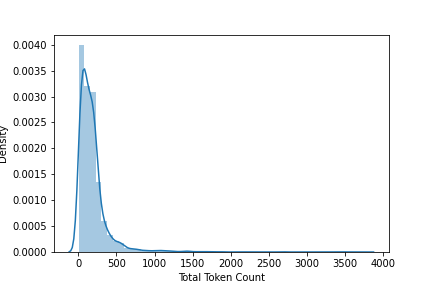
\includegraphics[width=\columnwidth]{total_length_dist}
  \caption{Distribution plot of combined token lengths}
  \label{fig:tdist}
\end{figure}

As seen from \cref{fig:tdist}, the token length can be capped at 512 and we should still preserve the discourse captured in the set of tweets.
However, in order to maximise the information used by the BERT model, stopwords were removed as well. 

\subsubsection{Model}
The model was developed using PyTorch \cite{pytorch} and trained via a TPU instance on Google Colab first. 
The Google Colab based training failed to train after a certain amount of time, this was due to the fact that Google Colab times out 
sessions after a small period (relative to the training time) of time. In order to combat this

%%%%%%%%%%%%%%%%%%%%%%%%%%%%%%%%%%%%%%%%%%%%%%%%%%%%%%%%%%%%%%%%%%%%%%%%%%%%%%%%%
%%% OTHER SECTION 1
%%%%%%%%%%%%%%%%%%%%%%%%%%%%%%%%%%%%%%%%%%%%%%%%%%%%%%%%%%%%%%%%%%%%%%%%%%%%%%%%%

%%%%%%%%%%%%%%%%%%%%%%%%%%%%%%%%%%%%%%%%%%%%%%%%%%%%%%%%%%%%%%%%%%%%%%%%%%%%%%%%%
%%% OTHER SECTION 2
%%%%%%%%%%%%%%%%%%%%%%%%%%%%%%%%%%%%%%%%%%%%%%%%%%%%%%%%%%%%%%%%%%%%%%%%%%%%%%%%%


\nocite{burchell}
\nocite{ma_gao_wong_2018}
\nocite{baris_schmelzeisen_staab_2019}
\nocite{Gardner2017AllenNLP}

\bibliographystyle{acl_natbib}
\bibliography{main}

%\appendx



\end{document}
